\documentclass{report}
\usepackage[english]{babel}
\usepackage{latexsym}
\usepackage[usenames,dvipsnames]{color}
\usepackage{verbatim}
\usepackage[pdftex]{hyperref}
\usepackage{graphicx}
\begin{document}
\thispagestyle{empty}
\begin{center}
\Huge{Gridmaker}\\
\LARGE{User manual}\\
\vfill
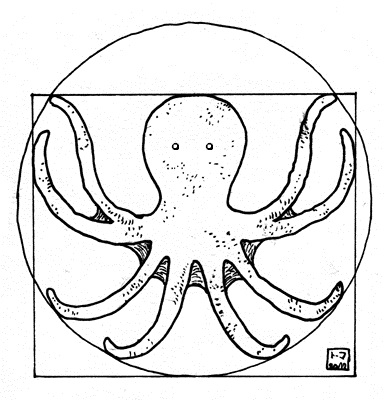
\includegraphics[width=0.7\textwidth]{vitruve_octopus.jpg}\\
\vfill
version 1.6 - 21/02/2013\\
\vfill
\large Julien Dorval
\end{center}
\tableofcontents

\chapter{Introduction}
\section{What is Gridmaker ?}

Gridmaker is a set of programs and scripts made to build a grid of stellar models with the evolution code MESA. Gridmaker takes a set of metallicities,
masses and mixing lengths, run MESA over each combination and writes all the output on a single HDF5 archive. This software was built between October 2012 and February 2013
at the School of Physics, University of Sydney by Julien Dorval. For Gridmaker to be useful, a multicore machine is necessary. The code was developped on the machine 'extend'
which is a 40 cores server running Linux.

\section{What is MESA ?}

MESA is an open source stellar evolution code which enables simulation/modeling of state-of-the-art equation of state, opacity, nuclear burning and element diffusion as stand 
along modules or integrated in MESA-star as a stellar evolution code. It also handles accretion, mass-loss, rotation and magnetic fields.
It is a very powerful code. For example, it evolves a ball of interstellar gas all the way to the WD cooling sequence with no interaction from the user, it can be used to model
 brown dwarfs and giant planets, and it can be used to model supernova progenitors.
MESA is user friendly and and one can literaly start using it straight after installation. There is a large community of users and developers which provide
a good support for new users. 

\section{What is HDF5 ?}
HDF5 is a data model, library, and file format for storing and managing data. It is designed to allow for fast, easy access and managing of very large datasets.
It also compresses the data. Functions in several languages exist to create, write, and read HDF5 files, as they can't be accessed directly.


\chapter{How to use Gridmaker}

\section{System configuration}

Before starting to use Gridmaker, you should set up your system to install MESA and HDF5. Detailed instructions to install and use MESA can be found
on the MESA website: \url{http://mesa.sourceforge.net/}. You should include these in your .cshrc file:
\begin{verbatim}
setenv MESASDK_ROOT ~/mesasdk
source $MESASDK_ROOT/bin/mesasdk_init.csh
source /usr/physics/idl8/idl/idl/bin/idl_setup
setenv MESA_DIR [*path to MESA in your system*]/MESA_4631/mesa
\end{verbatim}
You should as well include the path to HDF5 so you can compile the C program:
\begin{verbatim}
set path=( /usr/physics/hdf5/bin $path )   
\end{verbatim}
I am writing these for information, but it is strongly advised for any beginner to seek help from an experienced MESA user, and/or someone with HDF5 experience. Don't forget to change the path to MESA if you install a new version. Finally, you need to have access to the zams directory, where all the MESA starting models are stored. They currently can be found at 
\begin{verbatim}
/import/extend2/dorval/MESA/MESA_4522/zams
\end{verbatim}


\section{Install Gridmaker}

Gridmaker is available as a .tgz file, which is a tarball, an archive. It is extracted through:
\begin{verbatim} tar -zxf [name of archive]
\end{verbatim}
You now have a directory named \verb+gridx.x+ with \verb+x.x+ depending on the version you have. This directory contains all the files and directories needed to run Gridmaker (except the zams models). Gridmaker needs to be run from this directory. If you already have installed MESA, you can go 
to the \verb+gridx.x/tube1+ directory and build the MESA files by launching \verb+./mk+ . If in your version, \verb+hdf5_processing/hdf5_maker+ 
doesn't exist, you should build it by going into \verb+hdf5_processing/+ and launch the makefile with \verb+make+. You will need to have HDF5 
installed and added to your path for the makefile to work. The last thing is to configure the parameters.txt. Three paths are defined, you should 
set the global path and output path to the present grid directory ([..]/gridx.x), and make sure the path to the zams directory is valid and that it contains all the starting models for each metallicity that you want. Once both MESA \verb+star+ and \verb+hdf5_maker+ are built, Gridmaker is configured and ready to run ! 

\section{Quick start}

The input parameters for Gridmaker are the sets of metallicities, masses and mixing lengths that you want to use. These are text files whose names are listed in parameters.txt. In the default configuration, their names are metal.list (2 metallicities), mass.list (4 masses) and mixing.list (1 mixing length). This is a test configuration, which will make Gridmaker run for about 2 minutes. To test it, open IDL, place yourself in the grid directory, compile \verb+grid_creator.pro+ and launch it with the parameters file as an argument:

\begin{verbatim} IDL> grid_creator, 'parameters.txt' [, /overwrite]\end{verbatim}

\paragraph{} The overwrite keyword means you want to replace any existing HDF5 file, if you're not setting it, you will only add the data to the existing file. For a first try, since there is no existing file yet, you can use the procedure without the keyword. If Gridmaker was correctly installed, you should not see any error message. MESA will create 'tube2' and 'tube3'. These are MESA directories, copies of tube1. Each tube runs one MESA process, the number of 'tubes' set in parameters.txt correspond to the number of parallel MESA runs, each of which can be allocated multiple cores. In the default configuration, there are 3 tubes with 2 cores each. tube1 already exists, so \verb+grid_creator+ will create two more. The program then launches one MESA run per tube using the first three combinations of parameters while displaying information on the run. Once the first tubes are launched, \verb+grid_creator+ waits for the MESA runs to finish. You can monitor the progress of the grid as a whole by looking at the progression file:\\ 
\begin{verbatim}
less progress/progression
\end{verbatim}
\paragraph{} Once one of the MESA runs ends one evolution track, \verb+grid_creator+ copy out the result in the \verb+output+ directory and signals the C program \verb+hdf5_maker+ that some new data is available. \verb+grid_creator+ then launches a new run with a new set of parameters in the tube that was running this evolution track.

\paragraph{} When \verb+grid_creator+ gives \verb+hdf5_maker+ data of a new evolution track, \verb+hdf5_maker+ reads this new data from the output directory and writes it to the hdf5 file. It then tells \verb+output_data_deletion+ to delete the MESA profiles for this stellar model in the output directory. \verb+output_data_deletion+ is a bash script running alongside \verb+grid_creator+ and \verb+hdf5_maker+. MESA (in the Gridmaker configuration) produces two files for each step of the evolution of a stellar model: profiles and fgong files. The profiles  are deleted because they take a lot of space and are written in the HDF5 file anyway, the fgong files are left as text files for later use by, for example, ADIPLS. You can monitor the progress of the HDF5 processing by looking at the dedicated logfile: 

\begin{verbatim} less hdf5_processing/logfile_hdf5
\end{verbatim}

\paragraph{} In this file, \verb+hdf5_maker+ writes any interesting information or problem about the process of writing the data into HDF5 format.

\paragraph{} Once Gridmaker is done (no more computing of models in the progression file, and "END found" in the hdf5 logfile), all the profiles and history files from MESA are contained in the test.h5 file in \verb+hdf5_processing/+ . 


An HDF5 reading IDL procedure(  is available in the main grid directory. It
shows how HDF5 data can be accessed and read into IDL variables.

\section{Configure Gridmaker}

\subsection{parameters.txt}

This file contains:
\begin{itemize}
\item[-] The name of the metallicity list
\item[-] The name of the mass list
\item[-] The name of the mixing length list
\item[-] The number of tubes which will be created and used
\item[-] The number of cores you want to allocate to each tube
\item[-] The path to your current grid directory
\item[-] The path to the output directory (should probably be IN the grid directory)
\item[-] The path to the ZAMS MESA models
\item[-] The name of the output HDF5 file, with the .h5 extension
\end{itemize}

\paragraph{} The .list files are simply one value per line, without any header or specific syntax. The grid creator will tell you if your choice of tubes
and cores adds up to more than 40 cores, which is what extend has. If you are working on fewer cores, you should change this number in the code of 
grid\_creator.pro . The paths should not have a '/' character at the end.


\subsection{shared\_inlist}

A MESA run takes a single file as a user input: the inlist. This file defines all the parameters, options, output format that MESA will use to make stellar models and write the data. The part defining the metallicity, mass and mixing length are managed by the grid creator. The rest of the inlist, which set a lot of things, comes from the \verb+shared_inlist+ file in the grid directory. This file will be copied into each tube and given the name \verb+inlist+. In this inlist file, there is a link to a file named \verb+inlist_parameters+, which is generated by grid\_creator and specifies the metallicity, mass and mixing length to use for each given run. To put it simply: \verb+shared_inlist+ defines the physics of the models, which will be shared by the whole grid, and \verb+inlist_parameters+ defines the physical parameters of each run.

\section{HDF5 structure}

\paragraph{}A HDF5 file's structure relies on groups. These behave like directories, and paths are similar to unix paths. Gridmaker produces a HDF5 file with a similar structure than the output directory: a first level with a directory per metallicity, then in these, one directory per stellar model. Masses and mixing lengths are on the same level, as the directories names for each model bear the two information. For example, the data for a star with a metallicity of 0.0001000, 0.50 solar masses and a mixing length of 1.80 will be found in:
\begin{verbatim}
0.0001000/M0.50_L1.80/
\end{verbatim}
\paragraph{}Two types of data can be found for each stellar model: the history data which contains the evolution of several global parameters over the evolution track, and the models data, in which spatial information on the star itself can be found for each step of its evolution. The history data has its own subfolder, as well as each model in the evolution. For example, if you want the evolution of log(Teff) over time from ZAMS to thermal pulse (or to the age of the universe if the model doesn't reach the pulses), this data can be found at this path, using the variable names used by MESA when printing the history.data file: 
\begin{verbatim}
0.0001000/M0.50_L1.80/history/age
0.0001000/M0.50_L1.80/history/log_Teff
\end{verbatim}

\paragraph{}If you now want to know how was log(T) as a function of log(P) in the star for the 14th model of the same evolution track, these can be found at:
\begin{verbatim}
0.0001000/M0.50_L1.80/14/logP
0.0001000/M0.50_L1.80/14/logT
\end{verbatim}

\paragraph{}Finally, history and model directories have attributes: scalar values attached to them, that can be read faster than actual datasets. The attribute of a history directory is called 'maxmodel' and is the number of the last model in the evolution track, which is normally the total number of models for this track. The attribute of a profile directory is called 'nzones' and is the number of spatial zones MESA defined in the star at this step in the evolution track.

All this data can be accessed through IDL functions. An IDL procedure, \verb+example_read_hdf.pro+, is available in the grid directory. It shows and demonstrates how HDF5 data can be read into IDL variables.





\section{Resuming Gridmaker}

If for some reason, Gridmaker was interrupted while it was computing a grid, there is a possibility to resume the process where it was stopped. Simply
open IDL in the grid directory, compile \verb+resume_grid.pro+ and launch it:

\begin{verbatim} IDL> resume_grid, 'parameters.txt', /check_flags
\end{verbatim}

This will start Gridmaker at the point where it stopped. The check\_flags keyword is a way to avoid launching MESA on tubes where MESA processes from
the previous Gridmaker run are still computing. The way Gridmaker launch MESA in the tubes ensure that a file named 'free' will appear in the tube when the MESA process ends. This keyword check for the presence of a 'free' file (what I call a free flag) in each tube. If at least one tube doesn't have a free flag, \verb+resume_grid.pro+ signals it and stop. The fact that after an interruption there is a tube that doesn't have a free flag in it perhaps means that MESA is still running in this tube. 

\paragraph{}If this happens, a look at the processes through the command \verb+top+ allows to check if MESA is still running somewhere. MESA processes are named 'star'. You wouldn't be able to tell where the process is running, just to see if there are MESA processes or not. If for some reason, all the tubes are indeed inactive even though one does not have a free flag, you can force the grid to resume by removing the keyword. It is advised to always set the check\_flags keyword first, and to remove it only if you are sure all the tubes are inactive. To have several MESA processes on the same tube can cause a lot of problems and is not easy to identify.


\chapter{Structure of the code}

Gridmaker works with 3 different programs running in parallel and communicating through text files:
\begin{itemize}
\item[-]{\textbf{grid\_creator.pro}} is the main program, it calls the others. This IDL procedure reads the parameters, creates the tubes, launch
MESA and when a star is done, it copies the data in the output directory.
\item[-]{\textbf{hdf5\_maker}} (a C program) copies the history files and profiles data from the output directory into the HDF5 file.
\item[-]{\textbf{output\_data\_deletion}} (a bash script) deletes the profiles in the output directory. 
\end{itemize}
The final output is the output directory containing the fgong files for each star and a hdf5 file containing the information from the profiles and 
the history files.

\section{grid\_creator.pro}

This procedure, as well as resume\_grid.pro which we will describe later, uses several functions defined in \verb+functions.pro+ . As explained in the quick start section, the overwrite keyword allows to erase any existing file with the same name that the one specified in parameters.txt. If you just want to complete the existing grid, you should not set the overwrite keyword and specifies the name of this existing file in parameters.txt.

\subsection{Important variables}

\paragraph{}The main idea of the grid creator is to keep track of what star is being computed and which one will come next. This is done thanks to \verb+n+ a global 
index. It goes from 0 to the total number of parameters combination. For example, in the test configuration with 4 masses, 2 metallicities and 1 mixing
length, n goes from 0 to 8. Each star, which has a unique combination of parameters, has its n index. Each time grid\_creator launches a new star, it 
increments n. This index is the ultimate reference to know which star we are dealing with. Functions like n\_z, n\_m and n\_l can give the parameters
of a star just from its n.

\paragraph{}An important element is the repartition array. Its size matches the number of tubes, and at any moment, it contains the n indexes of 
the stars being computed in the tubes: repartition[0] contains the n of the star being computed in tube1, repartition[7] the one in tube8, etc (there 
is no tube0). This array is printed as a text file each time a new MESA run is started on a tube, that way resume\_grid will know exactly where things
were interrupted.

\paragraph{}Another crucial array is execution\_time. This is a 2D array of the size (number of metallicity) x (number of masses x number of mixing lengths). It keeps track of the time each star takes to compute, containing 0 when the star has not been done yet. It is intensively used when updating the progression file. To group masses and mixing lengths in a single dimension here was a choice made to ease the printing of the array as text files (still to make resuming easier). Each metallicity has its execution times file, for example:
\begin{verbatim}
execution_times/times_0.0001000
\end{verbatim}

\subsection{Tube managing}

\paragraph{}As said earlier, a tube is an autonomous MESA working directory. They are created at launch and deleted when the grid is complete (except for tube1 which
is permanent). One can go into tube1 and use \verb+./rn+ to launch MESA on its own. In fact, all grid\_creator is doing is printing the parameters for a
star into \verb+inlist_parameters+ (as well as the path to the right ZAMS file), which will be included in \verb+inlist+, and use the \verb+./rn+ command thanks to the spawn IDL function. MESA then 
reads the inlist file, which is actually the shared\_inlist that was copied in all the tube at the beginning, and the parameters printed by IDL.

\paragraph{}grid\_creator knows when MESA is done thanks to the way the launch command was given. The exact line in grid\_creator (which is actually
in the launch\_tube function in functions.pro) is:
\begin{verbatim}
spawn,'cd '+path+'/tube'+strtrim(i,2)+';
       setenv OMP_NUM_THREADS '+strtrim(n_core,2)+';
       ./rn > logstorage ;
       touch free &'
\end{verbatim}
\paragraph{}This is all a single string, which becomes a single command, as written in a terminal. The different instructions are separated by ';'.
The first instruction place the terminal in the tube[i] directory. We then set the number of cores used by MESA to our choice. MESA is then launched
with all its output directed into a dummie file called logstorage. This file can be checked later on if there was a bug somewhere, but it is replaced
for each star. The last instruction is the key: touch creates a empty file. Since all this was launched as a single command, they are sequentially
executed, which means the free file won't be created until MESA is done. The grid creator then just have to watch the tube and check the existence of 
a file named 'free' (I call it a free flag).


\subsection{Displaying the progress}

\paragraph{}The idea of the progression file is to write the progression of a single metallicity in a file which has the .part extension. When all the metallicities
has been written as separate files, a \verb+cat+ command through the spawn function fuses them all together in the progression file, in which one 
metallicity becomes one line. The top of the progression file, which contains information about the global running time of Gridmaker, percentage of
completion, etc, is \verb+header.part+ and is took by the file fusion as well. The .part are updated by two IDL functions: update\_header and update\_z\_part.

\paragraph{}To easily get the number of completed star in a given metallicity, update\_z\_part uses the execution\_times array to look for non-zero execution times compared to the total number of stellar models in a metallicity. Only the metallicities where there is at least one star computing are updated. The completion of each metallicity is tracked by an array called "completed". It is an integer array as big as the metallicity array. It is only 0s at launch, and once a metallicity is done, the corresponding position in completed is switched to 1.



\section{hdf5\_maker}

\verb+hdf5_maker.c+ and \verb+functions.c+ are located at:

\begin{verbatim}
hdf5_processing/src/
\end{verbatim}

And the executable \verb+hdf5_maker+ is created in the hdf5\_processing directory. When grid\_creator detects that a star was computed by MESA, it copies the data out in the output directory, and append its parameters to this file:

\begin{verbatim}
hdf5_processing/todolist
\end{verbatim}

In this format:

\begin{verbatim}
Z0.0001000 M0.50 L1.80
\end{verbatim}

\paragraph{}\verb+hdf5_maker+ monitors the todolist file and detect when a new star is added to the list. It then goes read the history and profiles data in the output directory, and writes them to the HDF5 file. Once a star has been treated by \verb+hdf5_maker+, it increments \verb+star\_count+, a text file containing a single integer representing the number of stellar models read and treated by the program. This count file is read each time the program is launched, and if non zero, all the stars that were already treated are passed in todolist. Once again, this is to make resuming easier. When starting a new grid, star\_count should contain 0 and todolist should be an empty file.

\paragraph{}The program itself, \verb+hdf5_maker.c+, is short and only calls several functions defined in \verb+functions.c+. Both of these files are well commented, and one can start reading the \verb+hdf5_maker.c+ and understand what is going on. The main idea is to use characters as signals. \verb+hdf5_maker+ reads the todolist in a loop. When it finds a 'Z' it means a new stellar model was added, and that its parameters can be read after the 'Z' thanks to the format we defined. If it finds a 'E', that means 'END' appeared in the todolist. This is the normal way for the IDL program to tell hdf5\_maker to stop.

\paragraph{}Because the program works through an unconditionnal infinite loop (\verb+for(;;)+), two precautions were added:
\begin{itemize}
\item[-] If a file named 'STOP' appears in the hdf5 processing directory, the program stops.
\item[-] If todolist doesn't exist anymore, the program stops.
\end{itemize}

\paragraph{} Another precaution is a quality control function integrated to hdf5\_maker. The code looks at the data before it writes it into HDF5 format, and doesn't do it if it detects a problem with the data. These potential problems are:
\begin{itemize}
\item No history file was found. This means either there is no data at all or the name of the star directory is not what it should be
\item There are more than 40 missing profiles compared to what is in the history file
\item There are more than 40 missing fgong files compared to what is in the history file
\item The last log(dt) in the history file is less than -7. This most likely means the star had a convergence problem and stopped.
\item The difference between the number of the last model and the number of lines in the history files is greater than 30. This never happened to me but it could mean MESA has appended a new run to an existing history file.
\end{itemize}
\paragraph{} When one of these is found, hdf5\_maker passes the star and signals the problem in the logfile\_file.

\section{output\_data\_deletion}

This is a simple bash script which deletes the profiles in the output directory once hdf5\_maker wrote them into the hdf5file. When hdf5\_maker is done writing a data from a stellar model into HDF5 file, we already said it incremented star\_count, but it also adds the path to the data in the output directory into the \verb+tobedeleted+ file, located in the hdf5 processing directory as well. Example of the content of tobedeleted while Gridmaker is running:
\begin{verbatim}
/import/extend2/dorval/grid1.4/output/0.0001000/M0.50_L1.80
/import/extend2/dorval/grid1.4/output/0.0010000/M0.51_L1.80
\end{verbatim}
This script monitors the tobedeleted file in an infinite loop and when a new path is added, it deleted all the files beginning with m at this location. This is because in the present configuration of Gridmaker, profiles names are formatted in a specific way. For example the 17th model of an evolution track with 1.4 solar masses, 0.0165959 of metallicity and a mixing length of 1.80 will be named:
\begin{verbatim}
m0140.z0.0165959.a180.o000.17
\end{verbatim}
\paragraph{} output\_data\_deletion actually works a lot like hdf5\_maker: it monitors a list file, perform an action when a new item is added, then increments a count file (here, it is called \verb+deletion_count+) to keep track of what has already been done. For the tobedeleted example given above, deletion\_count would probably contain 2 (if the deletion of the second line is complete). It also has the same two precautions than hdf5\_maker about its infinite loop. A 'STOP' file appearing in the hdf5 processing directory will immediately stop the script, and output\_data\_deletion will stop if tobedeleted can't be found. The normal way to stop is, as for hdf5\_maker, to reach an 'END' in its list, tobedeleted. This is actually added by hdf5\_maker when it wrote everything to the HDF5 file.

To sum it up, \verb+grid_creator+ sets up MESA in the tubes, launches it, wait for the run to end, copies the data in \verb+output+, then adds the parameters of the new data into \verb+todolist+. There, \verb+hdf5_maker+ reads this data and writes it into the HDF5 file. Once it is done, it adds the path to the original data in \verb+output+ to \verb+tobedeleted+. \verb+output_data_deletion+ picks up that path and deletes all the profiles. This keeps on until \verb+grid_creator+ copies out the data of the last evolution track. It then adds 'END' to \verb+todolist+. When \verb+hdf5_maker+ is done writing everything to the HDF5 file and reaches the 'END' in \verb+todolist+, it appends another 'END' at the end of \verb+tobedeleted+. This finally stops \verb+output_data_deletion+.

\section{resume\_grid.pro}

This IDL procedure is very similar to grid\_creator, but instead of beginning a new grid, it picks up where the previous one was interrupted. This can be done because grid\_creator writes a lot of information as text files at any moment:
\begin{itemize}
\item[-] The execution times in \verb+execution_times/+
\item[-] The repartition of MESA jobs in each tube in \verb+repartition+
\item[-] The date and elapsed time since starting point in \verb+journal+
\end{itemize}

\paragraph{} The program reads all this information, cleans the existing tubes and launch back each job that was interrupted in each tube. It then resumes the normal flow of grid\_creator. The interruption is signaled in an interruption file named \verb+z_0.0000000.part+ located in the progress directory. This is a way to include the information in the progression file between the header and all the other metallicities. The interruption file contains the state of progress of the grid at the interruption, followed by the time of interruption and time or resuming.

\paragraph{} As explained in section 3.1.2, the IDL procedures (grid\_maker or resume\_grid) know when a MESA process stops by watching the appearance of free flags. After an interruption, there may or may not be free flags in all the tubes, and there may or may not be MESA processes still running. The \verb+check_flags+ keyword checks the existence of free flags everywhere and doesn't resume the grid if it finds a tube without a free flag. The user should manually check there are no running MESA 'star' processes on the tubes, through \verb+top+ or \verb+ps aux | grep star+, and kill the existing ones. If resume\_grid still refuses to start and you are sure no MESA processes are running on the tubes, you can remove the keyword and force the resuming. This was added because several MESA processes on the same tubes won't actually return an error, and it makes all the data from this tube useless.

\section{Scripts}

Gridmaker heavily relies on bash scripts to perform actions on files. There are a lot of them, here is an exhaustive list:\\
\textit{In the main grid directory}
\begin{itemize}
\item[-]\textbf{cleangrid} deletes all traces from a previous run. It can be very slow if the output directory contains a lot of data. If that's the case, my advice would be to rename the existing output directory, create a new empty one, and launch a parallel rm process on the old one.
\item[-]\textbf{fgong\_renamer} renames all the *.FGONG files or FGONG.* files into fgong.* at the path provided as an argument
\item[-]\textbf{inlist\_copier} copies the shared\_inlist into each tube with the name 'inlist'. Takes the number of tubes as an argument
\item[-]\textbf{make\_directory} if the name provided as an argument is already a directory, doesn't do anything, else creates it. 
\item[-]\textbf{make\_or\_replace} removes any existing directory with the provided name if there is one, and creates a new one. 
\item[-]\textbf{rm\_silent} removes any files with names beginning with the argument, without error messages if there are none.
\item[-]\textbf{tube\_copier} copies tube1 into as many tubes as required in the argument.
\item[-]\textbf{tube\_deleter} removes all the tubes except tube1
\end{itemize}

\textit{In the hdf5\_processing directory}
\begin{itemize}
\item[-]\textbf{output\_data\_deletion} was already described in section 3.2. It doesn't take any argument
\item[-]\textbf{reset} erases any traces of a previous run except the .h5 file.
\item[-]\textbf{reset\_overwrite} does the same and erase any .h5 file it finds
\item[-]\textbf{resume\_maker} removes termination strings at the end of todolist and tobedeleted. It used to be used by resume\_grid when processes were stopped by using termination strings instead of ./stop. It is still called as a precaution but should have no effect.
\item[-]\textbf{stop} creates a STOP file, waits 1 second and removes it. It is a simple and sure way to stop both hdf5\_maker and output\_data\_deletion.
\end{itemize}  

\paragraph{}All these scripts are launched by typing, for example, \verb+./cleangrid+ in the directory where the script is located. They all contain a quick explanation of their purpose as comments.

\chapter{conclusion}

\paragraph{}To end this manual, a few pieces of advice. First, when for some reason Gridmaker fails, crashes or something else, it is a good idea to make sure \verb+./output_data_deletion+ and \verb+./hdf5_maker+ processes stop as well. They should be stopped and relaunched when using grid\_creator, but one should make sure there are not copies of the processes piling up. The \verb+stop+ script should interrupt them, and one can check if such processes are running with the grep command associated with ps aux:
\begin{verbatim}
ps aux | grep bash
ps aux | grep maker
\end{verbatim}

\paragraph{}Then, I did my best to protect the user for hidden errors, problems happening without error messages which in the end make the whole grid useless. Nevertheless, one should be careful and regularly check the data in the HDF5 file in addition to check the progression file and HDF5 logfile. Problems with MESA itself can sometime be seen in the progression file if the minimum or maximum execution time seems weirdly high or low compared to the average.

\paragraph{}Finally, if you have any question concerning Gridmaker for which you did not find an answer in this manual, you can send me an email at dorvaljulien@gmail.com.

\paragraph{}Have fun!










\end{document}
